%! TEX program = xelatex
\documentclass[a5paper, twoside, 11pt]{article}

\usepackage{enumitem, amsmath, amssymb, tikz, fancyhdr, stackengine, graphicx, sectsty, pdfpages, tabularx}

\usepackage[top=18mm, inner=10mm, outer=9mm, bottom=17mm, headheight=14.5pt, headsep=3mm, footskip=7mm]{geometry}

    \usepackage[english, russian]{babel}    %% загружает пакет многоязыковой вёрстки
    \usepackage{fontspec}                  %% подготавливает загрузку шрифтов 
    \defaultfontfeatures[\rmfamily, \sffamily]{Ligatures={TeX}}  %% свойства шрифтов по умолчанию
    \setmainfont[Scale=.9]{PT Serif} %% задаёт основной шрифт документа
    \setsansfont[Scale=.9]{PT Sans} %% задаёт шрифт без засечек
    \setmonofont{Consolas}              %% задаёт моноширинный шрифт 

    \usetikzlibrary{arrows.meta}

    \usepackage{unicode-math}
    \setmathfont{[latinmodern-math.otf]}
    \setmathfont[range=\mathit/{latin,Latin}]{PT Serif Italic}
    %\setmathfont[range=\mathit/{greek,Greek}]{Arno Pro}    
    \setmathfont[range=up]{PT Serif}
    \setmathfont[range="2264-"2265]{PT Serif}
    \setmathfont[range="003C-"003E]{PT Serif}
	
    \allsectionsfont{\sffamily}

    \usepackage{verbatim}
    \usepackage{import}

    \setlist[enumerate,1]{nolistsep}
    \setlist[itemize,1]{nolistsep}

    % русские названия заголовков разделов 
    \newcommand{\problemsname}{Задачи}
    \newcommand{\solutionsname}{Решения}
    \newcommand{\inputname}{Формат входных данных}
    \newcommand{\outputname}{Формат выходных данных}
    \newcommand{\examplename}{Пример входного и выходного файлов}
    \newcommand{\examplesname}{Примеры входного и выходного файлов}
    \newcommand{\commentsname}{Комментарии}
    \newcommand{\evaluationname}{Описание системы оценивания}
    \newcommand{\InputFileName}{input.txt}
    \newcommand{\OutputFileName}{output.txt}
    \makeatletter
    \def\kw@Explanation{Пояснение к примеру}
    \def\kw@Explanations{Пояснения к примерам}
    
    % заголовки разделов и~столбцов таблицы примеров
    \newcommand{\problempartheading}[1]{\par\medskip\noindent\textbf{\sffamily #1}\par\penalty10000\noindent}    
    \newcommand{\InputFile}{\problempartheading{\inputname}}
    \newcommand{\OutputFile}{\problempartheading{\outputname}}
    \newcommand{\Comments}{\problempartheading{\commentsname}}
    \newcommand{\Scoring}{\problempartheading{\evaluationname}}
    \newcommand{\Example}{\par\medskip\noindent\textbf{\sffamily\examplename}\raisebox{-2pt}{\strut}\par\penalty10000\noindent}
    \newcommand{\Examples}{\par\medskip\noindent\textbf{\sffamily\examplesname}\raisebox{-2pt}{\strut}\par\penalty10000\noindent}
    \newcommand{\Explanation}{\problempartheading{\kw@Explanation}}
    \newcommand{\Explanations}{\problempartheading{\kw@Explanations}}


	% русские знаки нестрогих неравенств
    \renewcommand{\geq}{\geqslant}
    \renewcommand{\leq}{\leqslant}
    \renewcommand{\ge}{\geq}
    \renewcommand{\le}{\leq}

    % штрафы за разрыв строки по оператору
    \binoppenalty=10000
    \relpenalty=10000
    
    \makeatletter
    % задача = \begin{problem}{name}{in}{out}{TL}{ML}
    \newenvironment{problem}[5]{%
\subsection{#1}%
\renewcommand{\InputFileName}{#2}%
\renewcommand{\OutputFileName}{#3}%
}{}
    \newenvironment{tutorial}[1]{\subsection{#1}}{}
    \renewcommand{\thesubsection}{\Alph{subsection}.}
    \renewcommand{\thesection}{}

    % ширина таблицы примеров - по умолчанию равна ширине текста минус 2 красных строки
    \newlength{\ex@mpwidth}
    \setlength{\ex@mpwidth}{\textwidth}
    \advance\ex@mpwidth-2\parindent
    \advance\ex@mpwidth-4\tabcolsep

    % ширины колонок ввода, вывода и~примеров для таблиц примеров
    \newlength{\ex@mpinpwidth}
    \newlength{\ex@mpoutwidth}
    \newlength{\ex@mpcomwidth}

% -- Setup sizes --
\newlength{\thelinewidth}
\thelinewidth=\textwidth
\newlength{\exmpwidinf}
\newlength{\exmpwidouf}
\newlength{\exmpwidewid}
\newlength{\exmpthreewidinf}
\newlength{\exmpthreewidouf}
\newlength{\exmpthreewidnote}

\newif\ifintentionallyblankpages

\exmpwidinf=0.43\thelinewidth
\exmpwidouf=0.43\thelinewidth
\exmpwidewid=0.9\thelinewidth
\exmpthreewidinf=0.28\thelinewidth
\exmpthreewidouf=0.28\thelinewidth
\exmpthreewidnote=0.30\thelinewidth


    % во всех примерах нужно следить за разрывами строк, вставлять знак комментария после завершения команды \exmp во избежание ненужных разрывов
    % например \exmp{2 4}{3 5}%

    
    % таблица примеров с 2 колонками (ввод и~вывод)
% :FIXME:

% This is magic, which delete space after verbatiminput
\addto@hook{\every@verbatim}{\topsep=0pt\relax}

\def\s@tm@cr@s{
    \def\widthin##1{\exmpwidinf=##1\relax}
    \def\widthout##1{\exmpwidouf=##1\relax}
    \def\stretchin##1{\advance\exmpwidinf by ##1\relax}
    \def\stretchout##1{\advance\exmpwidouf by ##1\relax}
    \@ifstar{
        \error Star must not be used in example environment any more
    }
}


\newenvironment{example}[1][]{
    \s@tm@cr@s#1
    \ttfamily\obeylines\obeyspaces\frenchspacing
    \newcommand{\exmp}[2]{
        \begin{minipage}[t]{\exmpwidinf}\rightskip=0pt plus 1fill\relax##1\medskip\end{minipage}&
        \begin{minipage}[t]{\exmpwidouf}\rightskip=0pt plus 1fill\relax##2\medskip\end{minipage}\\
        \hline
    }

    \newcommand{\exmpfile}[2]{
       \exmp{
          \verbatiminput{##1}
       }{
          \verbatiminput{##2}
       }%
    }


    \begin{tabular}{|l|l|}
        \hline
        \multicolumn{1}{|c|}{\bf\texttt{\InputFileName}}&
        \multicolumn{1}{|c|}{\bf\texttt{\OutputFileName}}\\
        \hline
}{
    \end{tabular}
}

    
    % таблица примеров с 3 колонками (ввод, вывод, комментарий), три аргумента - доли колонок 
        \newenvironment{examplecommented}[3]{
        \setlength{\ex@mpinpwidth}{#1\ex@mpwidth}
        \setlength{\ex@mpoutwidth}{#2\ex@mpwidth}
        \setlength{\ex@mpcomwidth}{#3\ex@mpwidth}
        \newcommand{\exmp}[3]{\begin{minipage}[t]{\ex@mpinpwidth}\raggedright\ttfamily ##1\medskip\end{minipage} &
                              \begin{minipage}[t]{\ex@mpoutwidth}\raggedright\ttfamily ##2\medskip\end{minipage} &
                              \begin{minipage}[t]{\ex@mpcomwidth} ##3\medskip\end{minipage}\\\hline%
        }
        \obeylines\obeyspaces\frenchspacing

        \noindent\begin{tabular}{|l|l|l|}
        \hline\multicolumn{1}{|c|}{\bf\texttt{\InputFileName}}&\multicolumn{1}{c|}{\bf\texttt{\OutputFileName}}&
        \multicolumn{1}{c|}{\bf\texttt{\commentsname}}\\
        \hline
        }{\end{tabular}\smallskip}

    
    % таблица примеров в~1 колонку. Один пример верстается в~4 строки (считая заголовки) на всю ширину таблицы
        \newenvironment{examplewide}{
        \advance\ex@mpwidth2\tabcolsep 
        \ttfamily\obeylines\obeyspaces\frenchspacing
        \newcommand{\exmp}[2]{
            \begin{tabular}{|c|}
            \hline
            \multicolumn{1}{|c|}{\bf\texttt{\InputFileName}}\\
            \hline
            \begin{minipage}[t]{\ex@mpwidth}\rightskip=0pt plus 1fill\relax\raggedright ##1 \medskip\end{minipage}\\
            \hline
            \multicolumn{1}{|c|}{\bf\texttt{\OutputFileName}}\\
            \hline
            \begin{minipage}[t]{\ex@mpwidth}\rightskip=0pt plus 1fill\relax\raggedright ##2 \medskip\end{minipage}\\%
            \hline
            \end{tabular}\smallskip
        }
        }{}

   \makeatother

	% колонтитулы
    \pagestyle{fancy}
    \makeatletter
    \fancyhead[LE]{\small \@title }
    \makeatother
    \fancyhead[RE]{}
    \fancyhead[LO]{2016--2017 учебный год}
    \fancyhead[RO]{}
    
    \newcommand\olympiad{*** ОПРЕДЕЛИТЕ ОЛИМПИАДУ КОМАНДОЙ \textbackslash olympiad !!! ***}

    
    \AtBeginDocument{\sloppy}
    \newcommand*{\hm}[1]{#1\nobreak\discretionary{}%
{\hbox{$\mathsurround=0pt #1$}}{}}


\newcommand{\foreword}{
\noindent\centerline{\parbox{0.9\textwidth}{\centering\sloppy\textbf{\olympiad}}}

\medskip
\noindent\centerline{\textbf{Дорогие участники!}}
\medskip

Проверка ваших решений производится \emph{автоматически} на наборе тестов, учитывающем различные варианты исходных данных, чтобы система могла выставить наиболее объективную оценку.

Для каждого теста выполняется следующая процедура:
\smallskip
\begin{itemize}[nolistsep]
\item
Система создает входной файл с исходными данными теста.
\item 
Запускается ваша программа, которая должна прочитать этот файл и~записать ответ в выходной файл.
\item
Затем система проверяет созданный вашей программой файл и~выносит решение о его правильности. 
\end{itemize}

Именно поэтому ваша программа должна читать данные из файла, а не с клавиатуры, и вывод записывать тоже в файл. Ни в коем случае нельзя использовать ввод с клавиатуры (например, функцию \texttt{readkey} в Паскале), так как в этом случае ваша программа будет ждать ввода бесконечно (и будет снята с тестирования после превышения лимита времени). Также важно строго соблюдать формат выходного файла. 

Приведем простой способ чтения из файла и записи в файл на языке Паскаль:\\
\framebox{\parbox{\textwidth}{
\small\tt
\{ {\rm\textit{ в начале программы }}\/ \}\\
assign(input, 'taskname.in');  reset(input);\\
assign(output, 'taskname.out'); rewrite(output);\\
\{ {\rm\textit{ теперь обычные процедуры read, readln, write, writeln будут работать \\ с файлами, а не с клавиатурой / экраном}} \}\\
  …\\
\{ {\rm\textit{ в конце программы }}\/ \}\\
close(output);
}}

\bigskip
\noindent
Ко всем задачам предъявляются следующие технические требования:

\noindent\addstackgap[8pt]{
\begin{tabular}{@{}ll}
Имена входного и выходного файлов & \textbf{см. в примерах к~задаче}\\
Максимальное время работы на одном тесте & 1 секунда\\
Максимальный объем используемой памяти	& 256 мегабайт \\
\end{tabular}
}


\begin{center}
\textbf{Желаем удачи!}
\end{center}
}


\newcommand{\importpolygontex}[2]{
\graphicspath{{problems/#1/statements/russian/}}
\import{problems/#1/statements/russian/}{#2.tex}   
}

\newcommand{\importproblem}[1]{\importpolygontex{#1}{problem}}
\newcommand{\importtutorial}[1]{\importpolygontex{#1}{tutorial}}

\renewcommand{\olympiad}{XVIII Республиканская командная олимпиада школьников \mbox{по программированию}}
\fancyhead[LE]{XVIII Республиканская командная олимпиада школьников}
\fancyhead[RE]{}
\fancyhead[RO]{2020--2021 учебный год}
\fancyhead[LO]{}

\begin{document}


\pagestyle{empty}

\begin{flushright}
\it
Эффективная и слаженная\\
командная работа -- залог успеха!
\end{flushright}
{}\vskip-18mm


\includegraphics[scale=0.15]{logo.png}
\\[3cm]

\begin{center}
\huge
XVIII РЕСПУБЛИКАНСКАЯ \\КОМАНДНАЯ\\ОЛИМПИАДА ШКОЛЬНИКОВ \\
ПО~ПРОГРАММИРОВАНИЮ
\end{center}

\vfill
\centerline{Якутск}
\centerline{4--5 марта 2021 г.}
\newpage
\noindent XVIII Республиканская командная олимпиада школьников по программированию.~--- Якутск, 2021.
\\[5mm]
Сборник содержит условия задач XVIII Республиканской командной олимпиады школьников по программированию и возможные варианты решений. Олимпиада проводилась 4--5 марта дистанционно.
\vfill

{}\hfill © Авторский коллектив, 2021

\newpage

\includepdf{sponsors2021.pdf}

\newpage
\noindent
\section*{ОРГКОМИТЕТ ОЛИМПИАДЫ}
\addcontentsline{toc}{section}{Оргкомитет}
%\fancyhead[RO]{Оргкомитет олимпиады}
\thispagestyle{plain}

ГОЛИКОВ Алексей Иннокентьевич \\ 
\textit{заместитель ректора Северо-Восточного федерального \\
университета имени М.\,К. Аммосова по кадровой политике~--- \\
председатель}
\\[3mm]
ПАВЛОВ Василий Климович \\
\textit{ректор Малой академии наук РС\,(Я)~--- заместитель председателя}
\\[3mm]
ПЕТРОВА Дария Александровна \\
\textit{ведущий специалист департамента по гос. политике \\
общего образования, воспитания и дополнительного образования \\
Министерства образования и науки РС(Я)}
\\[3mm]
НИКОЛАЕВА Наталья Васильевна \\
\textit{доцент ИМИ СВФУ, заведующая кафедрой информатики \\
Малой академии наук РС\,(Я  )}
\\[3mm]
СЕМЕНОВА Галина Александровна \\
\textit{проректор по учебно-организационной и воспитательной \\ 
работе Малой академии наук РС\,(Я)} 
\\[3mm]
ОБУДОВ Владислав Антонович \\
\textit{диспетчер  Малой академии наук РС\,(Я)}
\\[3mm]

\newpage
\section*{ЖЮРИ ОЛИМПИАДЫ}
\addcontentsline{toc}{section}{Жюри}
%\fancyhead[RO]{Жюри олимпиады}
\thispagestyle{plain}

ПАВЛОВ Никифор Никитич \\
\textit{к. ф.-м. н., доцент кафедры <<Информационные технологии>>\\ ИМИ СВФУ --- председатель}
\\[2mm]
БУЛАТОВ Василий Алквиадович\\
\textit{разработчик ПО, Yandex Europe B.V.}
\\[2mm]
ГАВРИЛЬЕВ Валерий Валерьевич\\
\textit{разработчик ПО, ООО «Яндекс.Технологии»}
\\[2mm]
ЗЫКОВ Тимур Алексеевич\\ 
\textit{студент, Физтех-школа прикладной математики и информатики \\
Московского физико-технического института \\
(национального исследовательского университета)}
\\[2mm]
ИВАНОВ Виталий Витальевич\\
\textit{старший инженер-программист, ООО «Ай-Новус»}
\\[2mm]
ЛЕВЕРЬЕВ Владимир Семенович \\
\textit{старший преподаватель кафедры ИТ ИМИ СВФУ}
\\[2mm]
МАКАРОВ Денис Иванович\\
\textit{студент, факультет информационных технологий и программирования Университета ИТМО}
\\[2mm]
МЕКУМЯНОВ Семен Леонидович\\
\textit{аналитик, Pinely}
\\[2mm]
НИКИФОРОВ Дьулустан Васильевич \\
\textit{старший преподаватель кафедры ИТ ИМИ СВФУ}
\\[2mm]
НИКОЛАЕВА Наталья Васильевна \\
\textit{к. ф.-м. н., зав. кафедрой ИТ ИМИ СВФУ,\\
зав. кафедрой информатики МАН РС(Я)}
\\[2mm]
ОБУДОВ Владислав Антонович, \\
\textit{диспетчер  Малой академии наук РС\,(Я) --- секретарь жюри}
\\[2mm]
ПАВЛОВ Александр Викторович \\
\textit{к. ф.-м. н., разработчик, ИП Павлов А.В.}
\newpage\noindent
ПАРНИКОВ Василий Васильевич\\
\textit{студент, факультет информационных технологий и программирования Университета ИТМО}
\\[2mm]
СЕМЕНОВ Никита Сергеевич\\
\textit{студент, факультет компьютерных наук \\
Национального исследовательского университета \\
«Высшая школа экономики»}
\\[2mm]
ЭВЕРСТОВ Владимир Васильевич \\
\textit{старший преподаватель кафедры ИТ ИМИ СВФУ}



\newpage
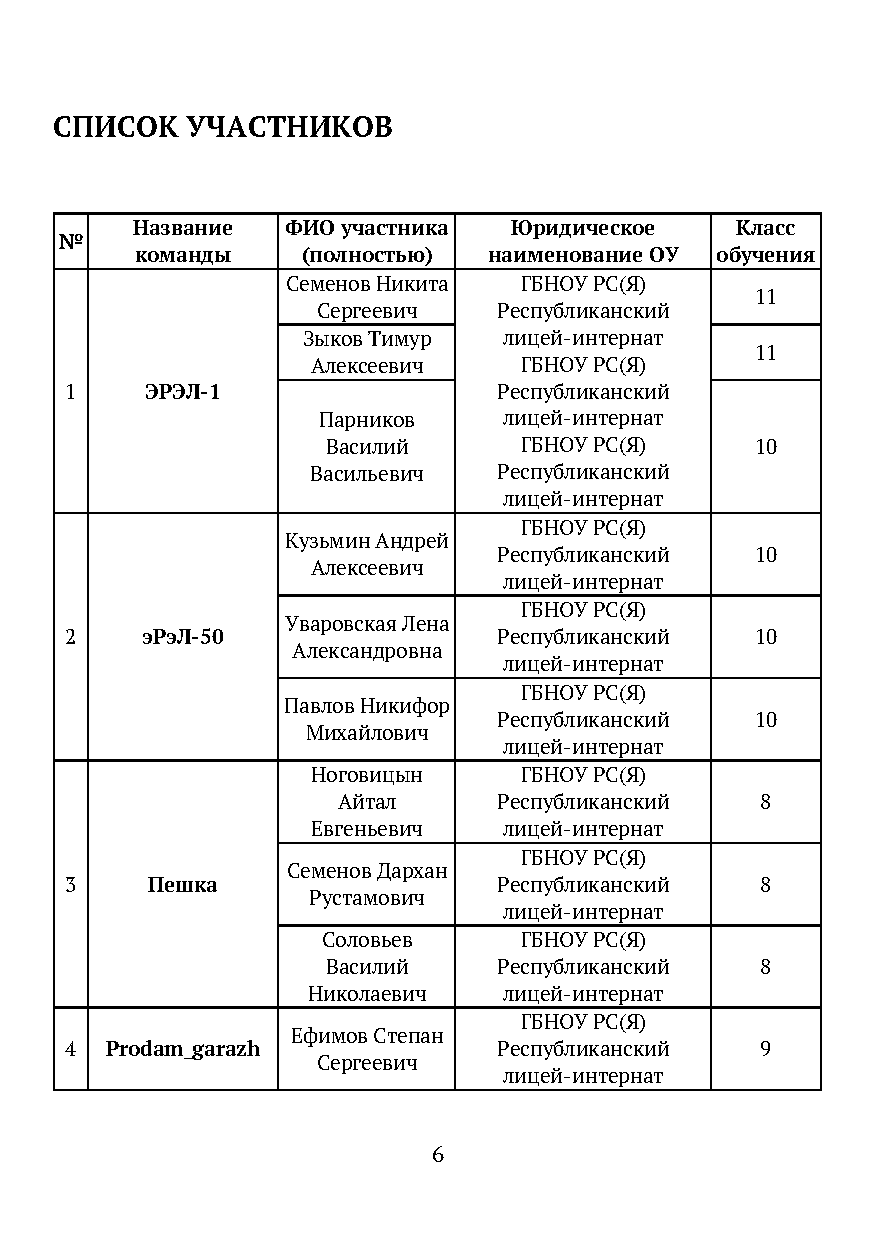
\includepdf[pages=-]{teamlist.pdf}

\pagestyle{fancy}

%=============================================================================
\newpage
\rm
\thispagestyle{plain}
\section*{УСЛОВИЯ ЗАДАЧ} 
\fancyhead[RO]{Условия задач}

\newcommand{\importproblem}[1]{
\graphicspath{{problems/#1/statements/russian/}}
\import{problems/#1/statements/russian/}{problem.tex}	
}

\importproblem{twice}

\importproblem{piston}

\importproblem{apes-king}

\importproblem{carpets}

\importproblem{numeral-system}

\importproblem{search-engine}

\importproblem{lights}

\importproblem{space-battle}

\importproblem{most-dangerous-individual}

\importproblem{air-raid}

\importproblem{graph-ways}


%======================================================================
\newpage
\fancyhead[RO]{Решения}
\section*{РЕШЕНИЯ} 
\setcounter{subsection}{0}


\newcommand{\importtutorial}[1]{
\graphicspath{{problems/#1/statements/russian/}}
\import{problems/#1/statements/russian/}{./tutorial.tex}	
}

\importtutorial{twice}

\importtutorial{piston}

\importtutorial{apes-king}

\importtutorial{carpets}

\importtutorial{numeral-system}

\importtutorial{search-engine}

\importtutorial{lights}

\importtutorial{space-battle}

\importtutorial{most-dangerous-individual}

\importtutorial{air-raid}

\importtutorial{graph-ways}



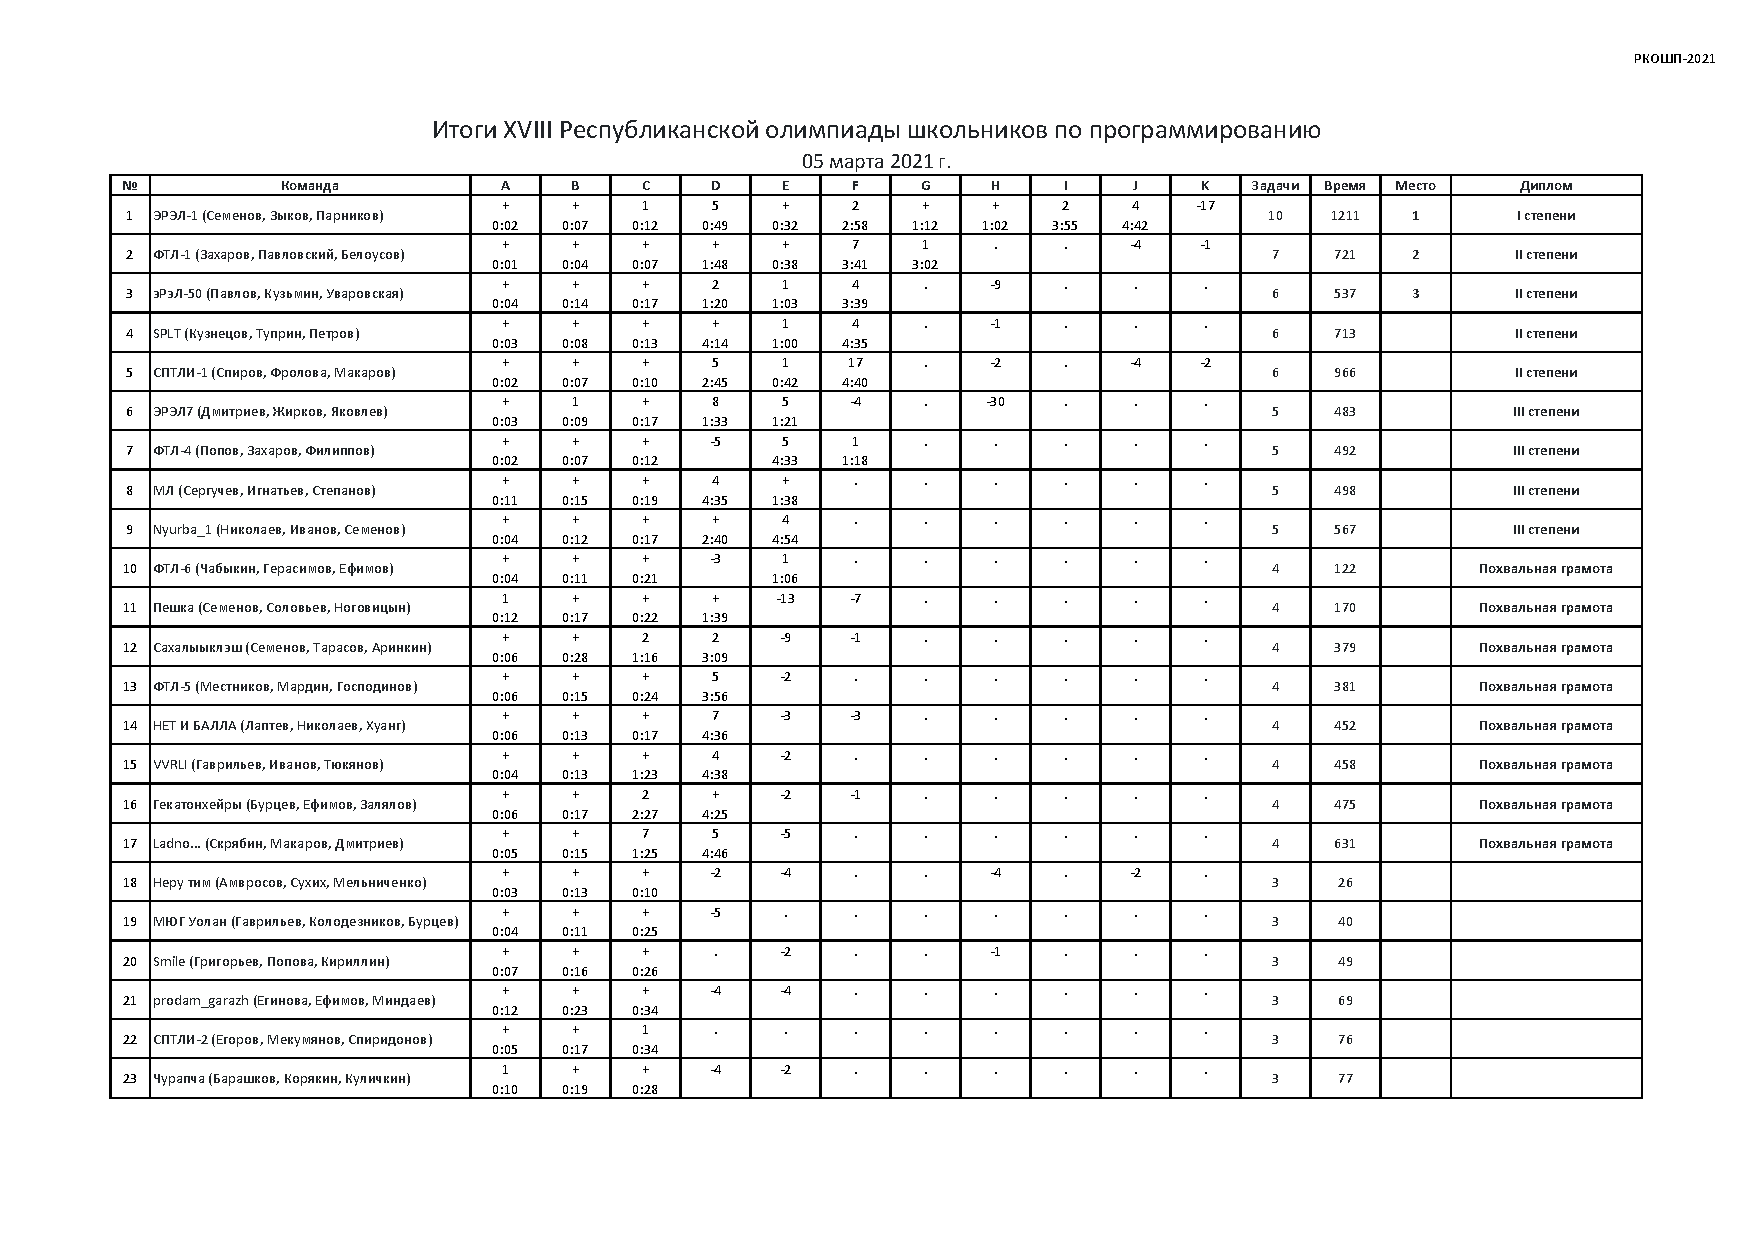
\includepdf[angle=90, pages=1-2]{results.pdf}


\end{document}